%---------- Quarto Capitulo ----------
\chapter{Ferramentas de desenvolvimento}\label{cha:ferramentas}
As organizações Google, Apple e Microsoft que desenvolvem os sistemas operacionais Android, iOS e Windows, respectivamente, oferecem aos desenvolvedores ferramentas e ambientes de desenvolvimento ricos em bibliotecas que fornecem suporte e facilidades no desenvolvimento de aplicativos.

\begin{figure}[h]
	\center
	\subfigure[fig:androidstudio][Android Studio]{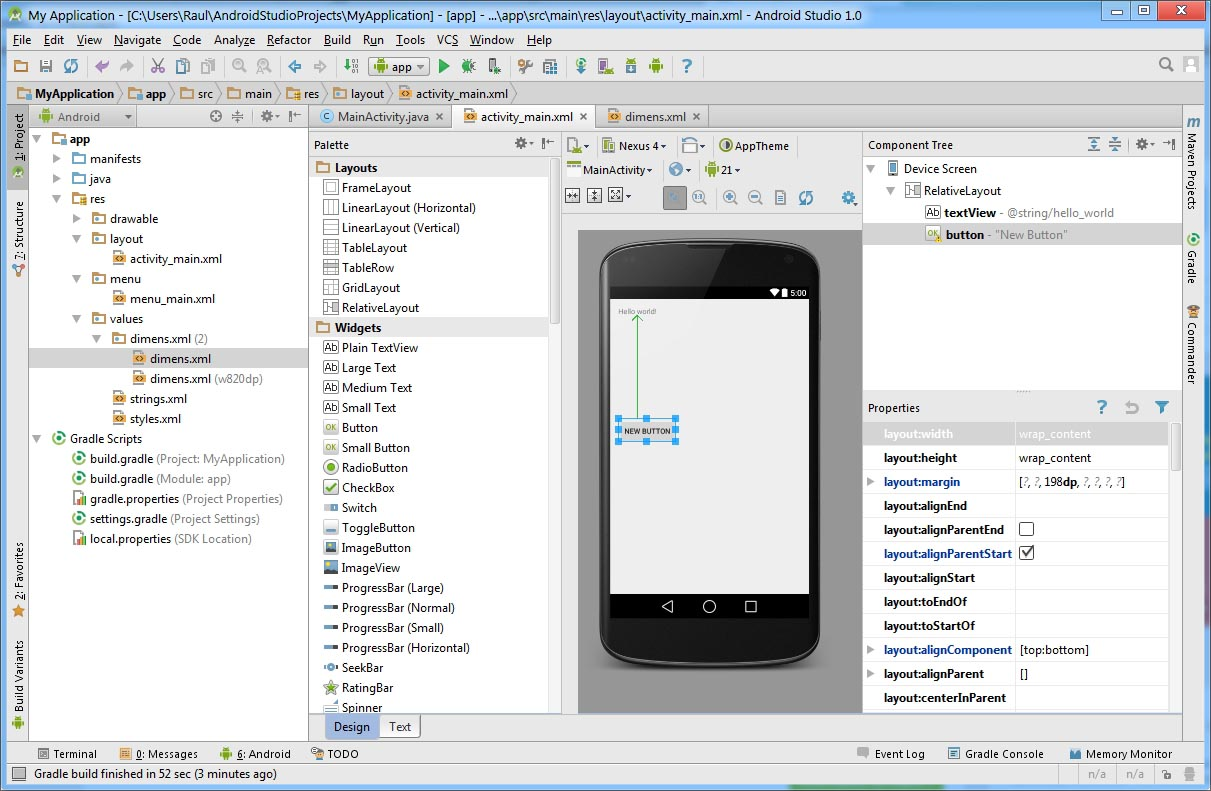
\includegraphics[width=7cm]{androidstudio.jpg}}
	\qquad
	\subfigure[fig:xcode][XCode]{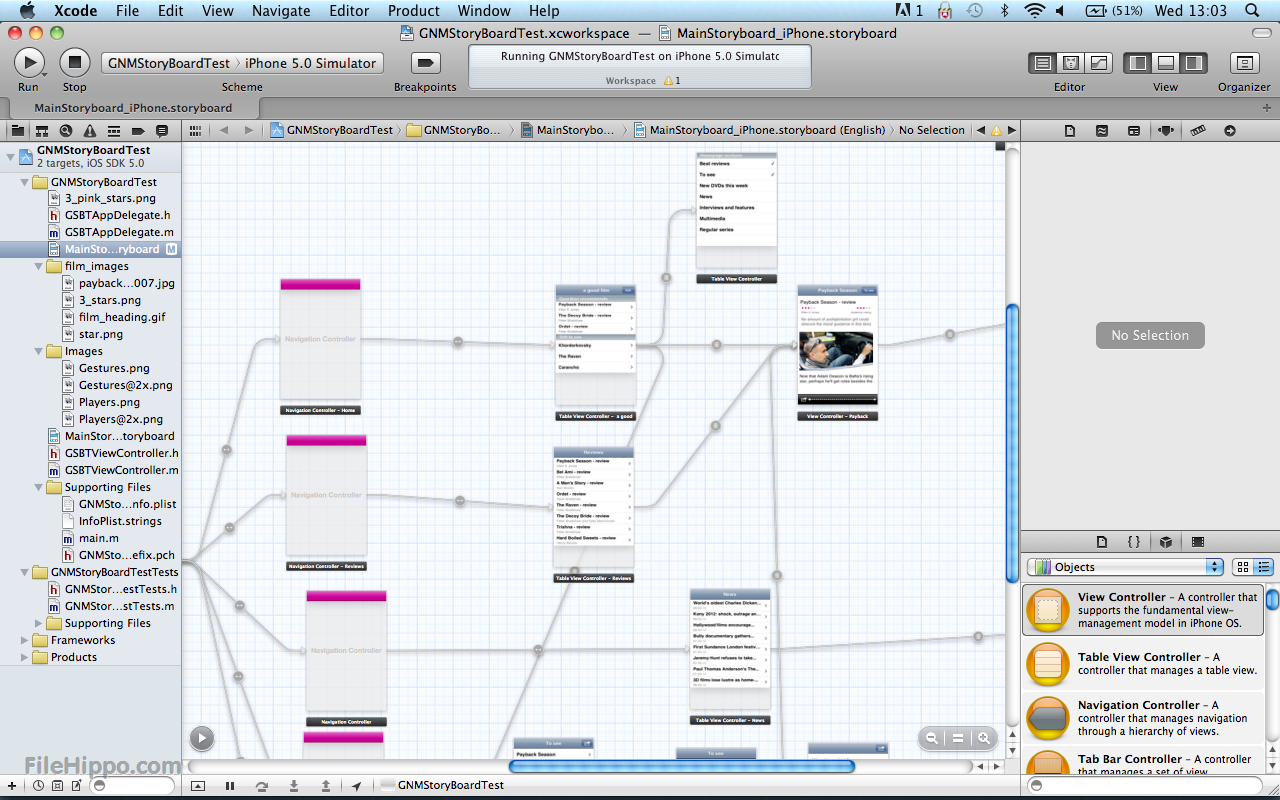
\includegraphics[width=7.5cm]{xcode.png}}
	\qquad
	\subfigure[fig:visualstudio][Visual Studio]{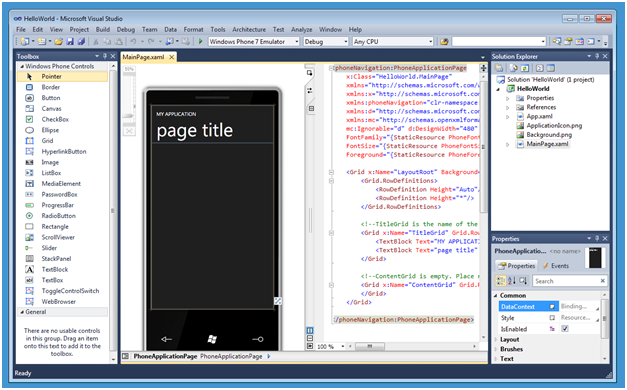
\includegraphics[width=7.3cm]{visualstudio.png}}
	\caption[IDE oferecidos pelas empresas]{\sigla{IDE}{Integrated Development Environment} oferecidos pelas empresas (a)Google, (b)Apple e (c)Microsoft}
	\label{fig:IDES}
\end{figure}
\vspace{-3mm}

Além das IDE (\textit{Integrated Development Environment}) apresentadas na Figura \ref{fig:IDES}, essas empresas também mantêm sites voltados aos desenvolvedores com documentos e informações sobre como utilizar as bibliotecas e as ferramentas para o desenvolvimento de aplicativos.

\section{Linguagens de Programação e Frameworks de Desenvolvimento}
Além das IDE e dos \sigla{SDK}{Software Development Kit} (\textit{Software Development Kit}) disponibilizados por essas empresas, outras organizações também desenvolvem tecnologias que apoiam a criação de aplicativos para essas platafomas como por exemplo as empresas Appcelerator e Apache. A Appcelerator disponibiliza um ambiente de desenvolvimento completo com IDE, plugins e bibliotecas conhecido como Titanium IDE, já a Apache disponibiliza ao desenvolvedores uma plataforma para criar aplicativos utilizando as tecnologias Javascript, \sigla{HTML}{Hyper Text Markup Language} (\textit{Hyper Text Markup Language}) e \sigla{CSS}{Cascading Style Sheets} (\textit{Cascading Style Sheets}) chamada Cordova.

Javascript é a linguagem com o maior número de repositórios ativos no GitHub, como mostrado na Figura \ref{fig:javascript}.

\begin{figure}[!htb]
	\centering
	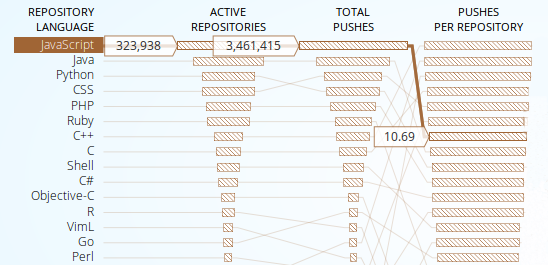
\includegraphics[width=.8\textwidth]{javascript-st.png} % <- formatos PNG, JPG e PDF
	\caption[Linguagens com maior número de repositórios ativos no GitHub]{Gráfico sobre as linguagens com repositórios ativos no GitHub. Fonte: \cite{githut}}
	\label{fig:javascript}
\end{figure}
\vspace{-3mm}

Com esse grande número de repositórios, a linguagem Javascript torna-se uma opção muito atrativa na escolha como linguagem principal no desenvolvimento de aplicativos, pois existem muitas pessoas utilizando a linguagem e isso faz com que seja fácil de encontrar exemplos de uso de código, existe a facilidade na obtenção de respostas de dúvidas em foruns de discussão, e também acontece o aumento na quantidade de bibliotecas utéis que podem ser utilizadas em diversos tipos de projetos.

\subsection{\normalfont\itshape Frameworks utilizando Apache Cordova}
Várias outras organizações utilizam o Apache Cordova como núcleo em seus frameworks para o desenvolvimento de aplicativos para dispositivo móveis, como é o caso do Adobe PhoneGap, Intel XDK e Ionic Framework.

O Apache Cordova oferece uma camada entre as várias funcionalidades existentes nos dispositivos móveis.
\begin{citacao}
O Cordova fornece uma interface que permite a comunicação entre os componentes nativos e o seu \textit{plugin}. Isso possibilita a chamada das funcionalidades nativas através do Javascript. Idealmente, a \sigla{API}{Application Program Interface} (\textit{Application Program Interface}) Javascript para a invocação de código nativo seria consistente para múltiplas plataformas. \cite{cordova}
\end{citacao}

A documentação do Apache Cordova mostra como criar um projeto simples através de poucos comandos e um desses comandos é a adição das plataformas suportadas, onde o desenvolvedor pode adicionar plataformas alvo e no momento da compilação serão gerados artefatos que poderão ser instalados nas plataformas correspondentes.
A documentação também apresenta uma tabela que exibe quais são as plataformas suportadas e quais as funcionalidades nativas que podem ser chamadas através de seu plugin.
Na Tabela \ref{tab:cordova} é exibido um resumo da tabela do Cordova e como pode ser notado, são poucas as funcionalidades que não são suportadas, isso aumenta as chances do uso desse \textit{framework}, já que com uma única implementação podemos ter várias plataformas alvo.

\begin{table}[!htb]
	\footnotesize
	\centering
	\caption[Funcionalidades nativas suportadas pelo \textit{plugin} Cordova]{Algumas das funcionalidades nativas suportadas pelo \textit{plugin} Cordova}
	\begin{tabular}{*8{c|}}
		 & \textbf{FireOS} & \textbf{Android} & \textbf{Blackberry} & \textbf{Firefox OS} & \textbf{iOS} & \textbf{Ubuntu} & \textbf{Windows}\\ \hline
		Accelerometer & \checkmark & \checkmark & \checkmark & \checkmark & \checkmark & \checkmark & \checkmark\\ \hline \SPACE
		Camera & \checkmark & \checkmark & \checkmark & \checkmark & \checkmark & \checkmark & \checkmark\\ \hline \SPACE
		Compass & \checkmark & \checkmark & \checkmark & x & \checkmark & \checkmark & \checkmark\\ \hline \SPACE
		Status Bar & x & \checkmark & x & x & \checkmark & x & \checkmark\\ \hline \SPACE
		Geolocalization & \checkmark & \checkmark & \checkmark & \checkmark & \checkmark & \checkmark & \checkmark\\ \hline \SPACE
		Events & \checkmark & \checkmark & \checkmark & x & \checkmark & \checkmark & \checkmark\\ \hline \SPACE
		BatteryStatus & \checkmark & \checkmark & \checkmark & \checkmark & \checkmark & x & \checkmark\\
		\hline
	\end{tabular}
	\label{tab:cordova}
\end{table}
\vspace{-3mm}

As aplicações que são desenvolvidas com essas tecnologias funcionam sobre o navegador de Internet dos dispositivos, isso faz com que nem todo o tipo de aplicação possa se beneficiar dessas facilidades. Aplicações que necessitam de um desempenho maior deverão ser implementadas em código nativo.

\subsection{Javascript em qualquer lugar}
Javascript está se tornando muito popular também como linguagem de backend, com o Node.Js.

Logo abaixo é apresentado um exemplo de código Node.js. Esse pequeno trecho de código quando executado disponibilizá um servidor web que poderá manipular muitas conexões concorrentemente.
\begin{footnotesize}
	\begin{verbatim}
	  const http = require('http');
	  const hostname = '127.0.0.1';
	  const port = 1337;
	  http.createServer((req, res) => {
	    res.writeHead(200, { 'Content-Type': 'text/plain' });
	    res.end('Hello World\n');
	  }).listen(port, hostname, () => {
	    console.log(`Running at http://${hostname}:${port}/`);
	  });
	\end{verbatim}
\end{footnotesize}

Caso esse código seja executado e alguém aponte o navegador de internet para o endereço do servidor, ele apenas devolverá ao usuário a mensagem \textit{Hello World}. Nada muito útil, mas o que deve ser levado em consideração aqui é essa simplicidade e poder que o Node.js apresenta.
\begin{citacao}
Como um framework assíncrono dirigido a eventos, Node.js foi desenhado para contruir aplicações de rede escaláveis. A cada conexão uma chamada é disparada, mas se nenhuma requisição é feita o Node dorme. \cite{nodejs}
\end{citacao}

O Javascript pode ser encontrado até como linguagem auxiliar para manipulação de dados em Banco de Dados, como é o caso do MongoDB, um banco de dados orientado a documentos que utiliza o \sigla{JSON}{JavaScript Object Notation} (\textit{JavaScript Object Notation}) como estrutura de dados.
No SGBD desse banco de dados podemos utilizar funções Javascript sobre os dados retornados numa consulta.
\begin{citacao}
MongoDB faz com que trabalhar com banco de dados seja simples e elegante. Ele utiliza um modelo de dados JSON que é mapeado para a sua aplicação, e possui esquemas dinâmicos que permitem uma iteração muito rápida. Tem bibliotecas para a linguagem que você utiliza para codificar. E ele tem uma linguagem de consulta expressiva que lhe permite buscar, ordenar, agregar dados sem a necessidade de escrever código extra. Ele ainda é mais fácil de implantar, provisionar e escalar.\cite{mongodb}
\end{citacao}